\documentclass[11pt]{article}
\usepackage{graphicx}
\usepackage{fancyvrb}
\usepackage{comment}
\usepackage[paper=letterpaper,margin=1.0in,includehead=false,includefoot=false]{geometry}

\newcommand{\cursor}{%
\begin{center}
\marginpar{\vskip 4pt\sc Cursor}
\begin{tabular*}{\linewidth}{c}
\hline
\end{tabular*}
\end{center}
}

\DefineVerbatimEnvironment{Code}{Verbatim}{fontsize=\footnotesize,xleftmargin=5pt}
\DefineVerbatimEnvironment{SemiCode}{Verbatim}{fontsize=\small,commandchars=\+\{\}}

\begin{document}

\title{Embedded Domain Specific Languages inside Functional Languages}
\author{Andy Gill, University of Kansas}
\maketitle

\section{A Domain Specific Language}

There are many ways to give a computer instructions.
%
%% "might" might sound better than "may"
An electrical engineer might write a MATLAB program,
a database administrator may write an SQL script,
a hardware engineer may write in Verilog,
and an accountant may write a spreadsheet
with embedded formulas.
%
%% This sentence isn't clear, nor does it lead into the next sentence very well.
%% I'd suggest expanding on this point to make it clearer.
Aside from the difference in language, there is an
important difference in {\em form\/} and {\em idiom\/}.
%% Maybe you should emphasise "idiom" as well?
%
All of these examples use languages
customized to the job at hand, and build computational
requests in a form both familiar and productive
for the programmer (though an accountant may
not think of herself as a programmer.)
All these examples are use of domain specific languages.


A Domain Specific Language is a special purpose language,
designed to encapsulate possible computations in a specific
domain. Following our earlier examples of MATLAB, SQL,
%% earlier examples of?
Verilog, and spreadsheets, the domains would be scientific modeling,
database queries and updates, hardware circuits, and financial computations, respectively.
Considering SQL specifically, there is nothing SQL does that could not
be done in Java or C, or any other general purpose programming
language. SQL simply bundles the actions needed to
interact with a database into a useable language,
%% is useable the correct adjective here?  Java and C are useable languages too.
and the language becomes the interface to communicate requests
to the database engine.
To pick a concrete example,
consider the act of trying to list a dynamically updated leader-board
for an online programming contest:
\begin{Code}
SELECT ROUND(SUM(s.Score)) as ss, t.TeamName FROM Solution s -- an aggregate score and team name
   LEFT JOIN Team t ON SolutionTeam = TeamId                 -- where the team has the correct id
   GROUP BY s.SolutionTeam                                   -- grouped by team name
   ORDER BY ss DESC                                          -- ordered by score
   LIMIT 20                                                  -- returning the first 20
\end{Code}
In a handful on lines, this query performs a complex
database search, and some computation, finding
the names and aggregate scores of the top 20 teams.

There are two fundimental types of Domain Specific Languages
(Figure X).
%
The first, like the SQL example, is a first class language,
with its own compiler or interpreter, and is often used in
its own ecosystem. (Figure X, (1)) 
All the examples mentioned so far fall
into this categary. The primary difference between SQL and
(say) Java is one of scope and focus, though sometimes
DSLs grow to be as large are general purpose languages.
%
The other class of Domain Specific Languages are languages
embeeded inside another hosting language. Such languages
can have the look and feel of being their own languages,
but leaverage the host language to provide an exisiting
ecostructure and initial semantics. It is this second
class of DSLs we are interested in, and is the subject of
this paper.

\begin{figure}
((FIGURE ABOUT DSL))

\end{figure}

\section{Embedded DSLs}

An embedded DSL (EDSL) is a language inside a language.
An EDSL implemented as a library in a host language
that has the look, feel and semantics of its own language,
customized to a specific problem domain.
Haskell~\cite{Haskell98Book}, our functional language of choice, is a great host for EDSLs
because of flexible overloading, a powerful type system, and lazy semantics facilitating this.

As an example of Haskell, consider reversing a list in Haskell
\begin{Code}
reverse :: [a] -> [a]
reverse []     = []
reverse (x:xs) = reverse xs ++ [x]
\end{Code}

This is the complete defintion of reverse: reverse reverses any type of list (the first line);
the reverse of an empty list, written \verb|[]|, is an empty list;
and the reverse of an non-empty list is the reverse of the tail of a linked-list,
appended to the front of the list.

Using this consise syntax, Haskell specifically and the functional programming
community in general have taken the ideas
of EDSLs, which considerably lowered the costs of developing
and maintaining a DSL, and developed many, many of DSL 
which provide higher-level interfaces and abstractions for well-understood systems.

\subsection{QuickCheck}

As a first example of a EDSL, consider the challange of writing test cases.
Or more specifically, writing the {\em properties\/} that test cases need to satisfy.

\begin{Code}
-- The reverse of a reversed list is itself
prop_reverse (xs :: [Int]) = reverse (reverse xs) == xs
\end{Code}

\verb|prop_reverse| is itself a regular Haskell function,
that takes a list of Int, and returns a boolean, based
on the validity of what is being proposed, specifically
that is a two reverses cancel each other out. 
Here is the neat part -- \verb|prop_reverse| is {\bf also\/} a
domain specific statement, and as such can also be considered
a sub-language inside of Haskell itself.  This style
of using function, in this case function with names
prefixed with \verb|prop_|, taking a number of typed
arguments, and returning a conditional. The property
written in Haskell is also an Embeeded Domain specific
language for properties.

We can run our EDSL, using a function called \verb|quickCheck|:
\begin{Code}
Prelude Test.QuickCheck> quickCheck prop_reverse 
+++ OK, passed 100 tests.
\end{Code}
By running \verb|quickCheck| with our explicit and specific property,
we execute our ESDL inside Haskell. The quickCheck function
generates 100 test cases for our property, and exectutes
them on the fly. If they all hold, then the system prints
a message reflecting this.

In turns out that this sort of mini-language is really useful in practice.

((Go into my QC notes))

\cursor{}

\subsection{Lava}

\section{Example HDL DSL: Kansas Lava}
\label{sec:KansasLava}

To take another example, consider describing hardware.
Hardware description languages and functional languages have
long enjoyed a fruitful partnership.
{\bf Lava} is the name given to a class of Haskell DSLs
that implement a function-based version of the hardware description
language Ruby~\cite{Jones:90:Ruby,Hutton:93:RubyInterp}. Ruby, not to be confused with the
modern programming language with the same name, was based
on relations, not functions, and was inspired by
the seminal work in $\mu$FP~\cite{Sheeran:84:muFP}.

Kansas Lava~\cite{Gill:13:TypesKansasLava} is a Haskell-hosted DSL developed by the PI
that follows the Lava line of research.
It is a language for expressing gate-level circuits that can be compiled for FPGAs via VHDL.
Haskell abstractions allow the programmer to work at
a slightly higher level of abstraction, where the model
is one of recursive components communicating via synchronized streams.
Kansas Lava has been deployed for the generation of high-performance circuits for telemetry decoders,
though the model used is general.
It is a deep DSL, and therefore
has the associated restrictions.


\begin{figure}[!t]
  \centering
  \begin{minipage}{0.5\textwidth}
    \centering
    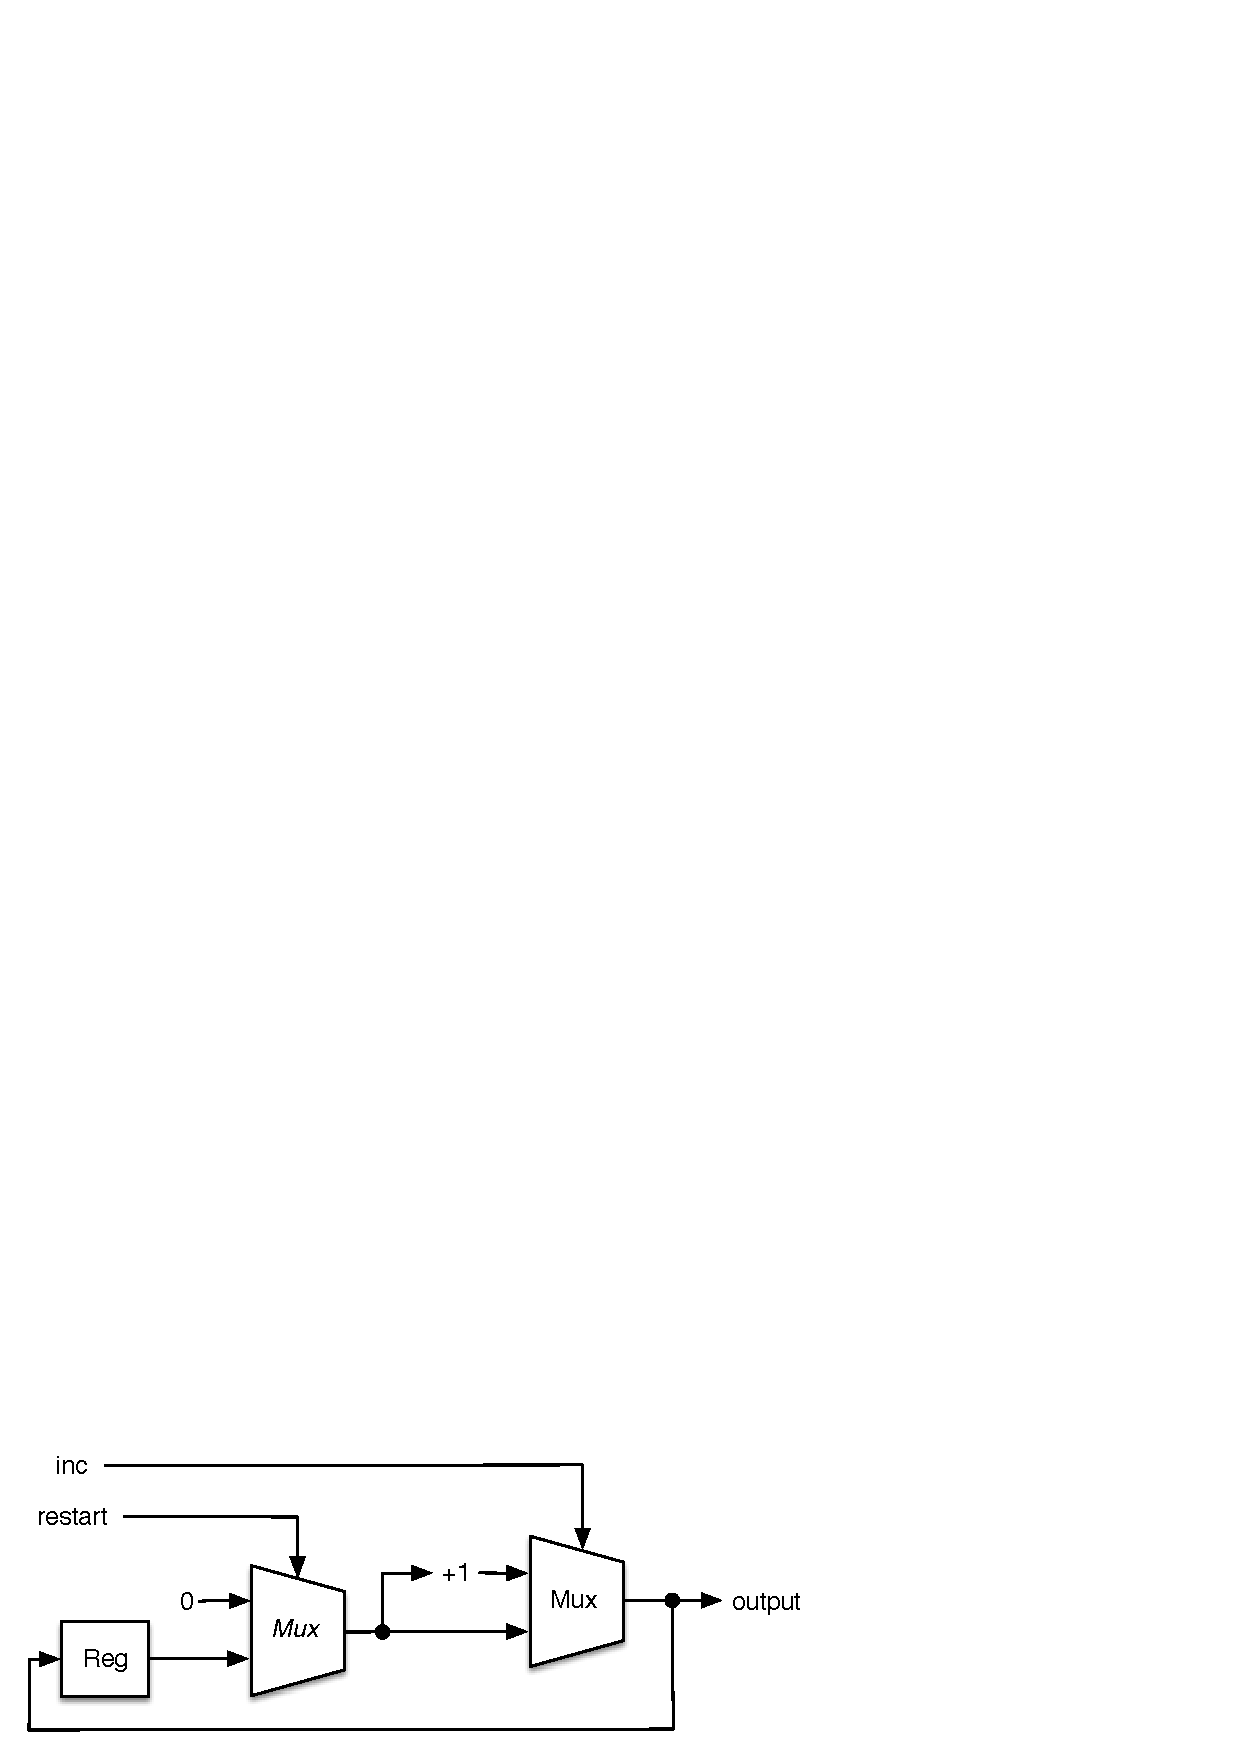
\includegraphics[width=0.8\textwidth]{images/Counter.pdf}
  \end{minipage}\begin{minipage}{0.5\textwidth}
     \centering
\footnotesize\begin{Code}[fontsize=\tiny]
entity counter is
  port(rst : in std_logic;
       clk : in std_logic;
       clk_en : in std_logic;
       restart : in std_logic;
       inc : in std_logic;
       output : out std_logic_vector(3 downto 0));
end entity counter;
architecture str of counter is
  signal sig_2_o0 : std_logic_vector(3 downto 0);
  ...
begin
  sig_2_o0 <= sig_5_o0 when (inc = '1')  else sig_6_o0;
  sig_5_o0 <= std_logic_vector(...);
  sig_6_o0 <= "0000" when (restart = '1') else sig_10_o0;
  sig_10_o0_next <= sig_2_o0;
  proc14 : process(rst,clk) is
  begin
    if rst = '1' then
      sig_10_o0 <= "0000";
    elsif rising_edge(clk) then
      if (clk_en = '1') then
        sig_10_o0 <= sig_10_o0_next;
  ....
end architecture;
\end{Code}
  \end{minipage}
  \caption{{\tt counter} Schematic and VHDL Generated by Kansas Lava}
  \label{fig:counter-picture}
%  \vspace{-0.1in}
\end{figure}

As an example of Kansas Lava, consider:

\begin{Code}

counter :: (Rep a, Num a, Clock clk, sig ~ Signal clk) => sig Bool -> sig Bool -> sig a
counter restart inc = loop
   where reg = register 0 loop
	 reg' = mux2 restart (0,reg)
	 loop = mux2 inc (reg' + 1, reg')
\end{Code}

This circuit connects two multiplexers,
an adder,
and a \verb|register|
to give a circuit that counts the number of
clocked pulses on a signal \verb|inc|.
The circuit takes two clocked signals,
and returns a clocked signal that explicitly
operates using the same clock, because they
share the same type.
Notice how the use of arithmetic is understated,
but simply uses (via overloading) the
standard syntax for addition; the {\tt Num}
constraint allows this.
Figure~\ref{fig:counter-picture} gives the
circuit intended for this description.

We can simulate sequential circuits with the
same directness as the combinational functions we invoked.
\begin{Code}
GHCi> toSeq (cycle [True,False,False])
T : F : F : T : F : F : T : F : F : ...
GHCi> counter low (toSeq (cycle [True,False,False]))
1 : 1 : 1 : 2 : 2 : 2 : 3 : 3 : 3 : ...
\end{Code}

We can also {\em reify\/} the circuit, into
a VHDL program. This is the key advantage and the
primary purpose of Kansas Lava. For example,
if we reify the counter with a width of 4 bits, we generate
the idiomatic but useable VHDL
listed in Figure~\ref{fig:counter-picture}.

As well as basic signal types,
we can build circuits that operate on Haskell
functions directly, provided the domain of the
function is finite. We use the \verb|Rep|
constraint to signify that we can enumerate
all possible representable values in a type,
giving the \verb|funMap| function.
\begin{Code}
funMap :: (Rep a, Rep b, Clock c, sig ~ Signal c) => (a -> Maybe b) -> sig a -> sig b
\end{Code}
The generated circuit is implemented using a ROM,
and we can generate control logic
directly in terms of Haskell functions
and data-structures. As a example, consider
a small ROM that stores the square of a
value.
\begin{Code}
squareROM :: (Num a, Rep a, Clock c, sig ~ Signal c) => sig a -> sig a
squareROM = funMap (\ x -> return (x * x))
\end{Code}
In this way, direct Haskell functions
can be lifted into the \verb|Signal| world.
Notice how the \verb|squareROM| function is
not specific about size but is
completely generic, only requiring the
type of the argument stream
to be representable as a number.

This use of a Haskell DSL for expressing circuits
is all well and good and {\em structural\/}.
But how can Kansas Lava be utilized to
describe more general forms of computation and parallelism?
Unfortunately at this point the model breaks down
to some degree. Programs can be written
that generate specific components, like ALUs,
but computation is more challenging to express
in Kansas Lava and other deep DSLs.


\subsection{Observations of Embedeed DSLs}

As can be seen, EDSLs are simply a way of thinking about a library.

Another observation to make regarding EDSLs is that
there are two flavors:
%% I don't like the use of ``First'' and ``Second'' in these bullet points.
\begin{itemize}
\item First, {\em DSLs that use a shallow embedding\/}, where values are computed with directly.
The result of a computation in a shallow DSL is a value.
\item Second, {\em DSLs that use a deep embedding\/} build an abstract syntax tree~\cite{Elliott:03:CompileDSEL-JFP}.
The result of a computation inside a deep DSL
is a structure, not a value, and this structure can be used to compute a value,
or be cross-compiled before being evaluated.
\end{itemize}
This is an important distinction. Historically, EDSLs have been shallow,
and as such are simply a ways of structuring an API to a library. Deep EDSLs
have the ability to {\em stage\/} code, that is executing a program
can generate another program, much like the well-known YACC DSL,
but at the cost of significantly restricting what forms of the DSL can
generate valid output from.
%% That sentence is a bit garbled.

To allow us to be more specific, we now
look at two case-studies:
\begin{itemize}
\item {\bf Kansas Lava} -- recent work by the PI on a hardware description DSL;
\item and {\bf Sunroof} -- a DSL for calling and creating JavaScript, also by the PI.
%% sunroof is your work too, right?
\end{itemize}
The unifying theme is that embedded DSLs can
be pragmatic, productive and useful. We present
these to allow us to make a technical argument that adding rewrite systems to
DSLs will improve their usefulness by removing
some of the inherent and outstanding shortcomings.

\section{Deep Embeddings of DSLs}

\section{Reification Tricks}

The process of extracting a structure from a deeply embedded ESDL
is called reification. 



 * running the description to get the AST 

\section{Use of Haskell’s type system for various things }

 * expression data type 
 * the phantom types trick 
 * Use of type classes (e.g. distinction of Seq and Comb in Signal) 
 * usefulness of laziness 
 * smart constructors ? 
 * sharing ?

%--------------------------------
% CAREER12


\section{Domain Specific Languages}








\end{document}
